\documentclass[english]{article}
\usepackage{fullpage}
\usepackage{amsmath}
\usepackage{tikz}
\usepackage{tkz-base}
\usepackage{graphicx}
\usepackage{algorithm}
\usepackage{algorithmicx}
\usepackage{algpseudocode}
\graphicspath{{../fig/}}

\usetikzlibrary{shapes,decorations,shadows}
\usetikzlibrary{decorations.pathmorphing}
\usetikzlibrary{decorations.shapes}
\usetikzlibrary{fadings}
\usetikzlibrary{patterns}
\usetikzlibrary{calc}
\usetikzlibrary{decorations.text}
\usetikzlibrary{decorations.footprints}
\usetikzlibrary{decorations.fractals}
\usetikzlibrary{shapes.gates.logic.IEC}
\usetikzlibrary{shapes.gates.logic.US}
\usetikzlibrary{fit,chains}
\usetikzlibrary{positioning}
\usepgflibrary{shapes}
\usetikzlibrary{scopes}
\usetikzlibrary{arrows}
\usetikzlibrary{backgrounds}
\tikzset{latent/.style={circle,fill=white,draw=black,inner sep=1pt, 
minimum size=20pt, font=\fontsize{10}{10}\selectfont},
obs/.style={latent,fill=gray!33},
const/.style={rectangle, inner sep=1pt},
factor/.style={rectangle, fill=black,minimum size=5pt, inner sep=1pt},
>={triangle 45}}

\pgfdeclarelayer{b}
\pgfdeclarelayer{f}
\pgfsetlayers{b,main,f}

\newcommand{\plate}[4]{
\begin{pgfonlayer}{b}
\node (invis#1) [draw, color=white, inner sep=6pt,rectangle,fit=#2] {};
\end{pgfonlayer}\begin{pgfonlayer}{f}
\node (capt#1) [ below left=0 pt of invis#1.south east, xshift=1pt,yshift=1pt] {\footnotesize{#3}};
\node (#1) [draw,inner sep=1pt, rectangle,fit=(invis#1) (capt#1),#4] {};
\end{pgfonlayer}
}


\newcommand{\shiftedplate}[5]{
\begin{pgfonlayer}{b}
\node (invis#1) [draw, color=white, inner sep=0 pt,rectangle,fit=#2] {};
\end{pgfonlayer}\begin{pgfonlayer}{f}
\node (capt#1) [#5, xshift=2pt] {\footnotesize{#3}};
\node (#1) [draw,inner sep=2pt, rectangle,fit=(invis#1) (capt#1),#4] {};
\end{pgfonlayer}
}

\usepackage[draft]{fixme}
\usepackage{babel}

\newcommand{\+}[1]{\ensuremath{\boldsymbol{\mathrm{#1}}}}

\begin{document}

\title{Bayesian Nonparametric Neural Image Segmentation}
\author{Kui Tang, $\sigma$(Joshua T.~Vogelstein, Jeff Lichtman, Bobby Kasthuri, Randal Burns, 
\\ Priya Manavalan) Frank Wood}
\date{\today}
\maketitle
\begin{abstract}
We develop a Bayesian nonparametric method to segment neurons in electron micrograph images of brain tissue. Our model imposes spatial locality on arbitrary features, automatically determines the number of segments in an image, and can be used in both unsupervised and semi-supervised settings. We introduce a novel geodesic distance feature which adaptively adjust segmentation to respect detected cell boundaries. Using data collected by Kasthuri et al., we show that our model can obtain plausible segmentations with no training data, while receiving a significant boost in its presence. Finally, our Bayesian nonparametric naturally extends to 3 dimensions, where neural columns of segments \emph{through} slices are modelled.
\end{abstract}

\section{Introduction}
A new branch of computational neuroscience, \emph{connectomics}, aims to reconstruct the physical location and circuit connectivity of the brain. Recent advances in electron microscopy have produced images of 10 nm in the lateral plane and 50 nm in the vertical plane, sufficient detail to capture most of even the smallest neural processes~\cite{Briggman2006}. The scale of the data is profound; the human brain is estimated to contain 100 billion neurons connected by up to a quadrillion synapses~\cite{Kasthuri2010}.

All published connectomes have been manually labelled. White et al. published the first connectome of \emph{C. elegans} in 1986, marking axons, dendrites, and cell bodies in each frame and tracing the labels through frames~\cite{White12111986}. Recent work in semi-automated methods are accurate and promising \cite{Roberts2011,Unger2009,Jarrell2012,Bock2011}, but current baseline speeds of computer-assisted manual tracing would still take 10,000 person-years to construct a mouse cortical column~\cite{Briggman2006}, hence the need for fully automatic methods.

EM images present several challenges for classical segmentation algorithm. First, structures or interest are small and densely packed \cite{Jain2007}. Second, due to the physical cutting process, images may be warped from slice to slice \cite{Koshevoy2006}.

\section{Related Work}
Automated techniques generally try to find cell boundaries---a highly distinctive feature. Because cells are usually disconnected, segmentation can be reduced to binary classification of whether voxels are inside or outside a cell. Segmentation can be done directlyin voxel space. Jain et al. \cite{Jain2007} achieved an 8.0\% test error with respect to hand-labelled ground truth with a convolutional neural network. This beats the 18.95\% error of thresholding; MRFs and CRFs do no better. Andres et al. obtain similar performance over the same dataset using the watershed algorithm over a probability map of a random forest with hand-engineered features \cite{Andres2008}. However, their dataset used a special intracellular stain which made segmentation easier. The generality of these solutions are thus unclear.

More common is to segment in pixel space and track the identity of segmented bodies in the vertical dimension. This mitigates the poor vertical resolution of EM images \cite{Kaynig2010, Briggman2006}. Jurrus et al. \cite{Jurrus2008} first obtain 2D segmentations with watershed after preprocessing, and construct a graph of segments across layers. Edges connect all segments that overlap in the plane, and weights favor segments with high cross-correlation low lateral displacement. Each neural process is a shortest path through this graph, computed by Dijkstra's algorithm. This cost function is robust to merging and losing of sections. But because Dijkstra's algorithm finds a single path, it cannot model branching. Kaynig et al. \cite{Kaynig2010a} presuppose segmentation and also represent the image as a graph of regions. Edge weights store pairwise features, and a random forest is trained to output a scalar similarity score for each pair. Then a probabilistic model encoding geometric constraints with cross-section correspondences as hidden variables is trained with EM. The maximum-likelihood result is the 3D reconstruction. These pairwise correspondences are fed to an agglomerative clustering algorithm, constructing the neural processes from ground-up in the same manner as a human. Unlike in Jurrus, processes may merge. However, each region is explicitly limited to two correspondences: one above and below, so processes still cannot branch.

Feature engineering significantly shapes the state of the art. Venkataraju et al. \cite{Venkataraju2009} generated 100 Hessian neighborhood features at each pixel and classified Jurrus's dataset with AdaBoost. Lucchi et al. \cite{Lucchi2010} develop ray descriptors, which capture shape features without a predefined shape model. These features are rotation, scale, and translation invariant, but strongly discriminate the types of objects observed in EM images. Their features were used in SVMs to classify interior and boundary points of mitochondria, considerably harder to classify than other cellular structures, and a graph cut found the final 2D segmentation with 98\% accuracy.

\fxwarning{Who cites Malik's normalized cuts?}

\section{Model and Features}
\label{sec:model}
\begin{figure}
\centering

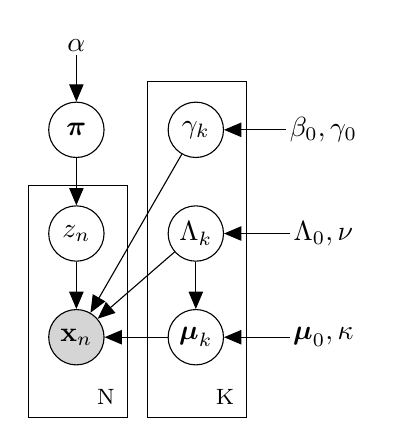
\begin{tikzpicture}
\matrix[row sep=6mm, column sep=8mm, matrix anchor=mid] (mdp) {
  \node (alpha) [const] {$\alpha$}; & & \\
  \node (pi) [latent] {$\+\pi$}; & \node (beta) [latent] {$\gamma_k$}; & \node (alphabeta) [const] {$\beta_0, \gamma_0$}; \\
  \node (z) [latent] {$z_n$}; & \node(Lambda) [latent] {$\Lambda_k$}; & \node(Lambdanu) [const] {$\Lambda_0, \nu$}; \\
  \node (x) [obs] {$\+x_n$}; & \node(mu) [latent] {$\+\mu_k$}; & \node(mukappa) [const] {$\+\mu_0, \kappa$}; \\
};

\draw [->] (alpha) -- (pi);
\draw [->] (pi) -- (z);
\draw [->] (z) -- (x);
\draw [->] (alphabeta) -- (beta);
\draw [->] (Lambdanu) -- (Lambda);
\draw [->] (mukappa) -- (mu);
\draw [->] (Lambda) -- (mu);
\draw [->] (beta) -- (x);
\draw [->] (Lambda) -- (x);
\draw [->] (mu) -- (x);

\plate{Nplate}{(z)(x)}{N}{}
\plate{Kplate}{(beta)(Lambda)(mu)}{K}{}

\end{tikzpicture}
\caption{The graphical model. Unlike a standard Gaussian mixture model, our model couples $\gamma_k$ and $\+\mu_k$ through the $\+x_n$, giving the flexibility to model boundary constraints, but also presents challenges in inference. See text for details.}\label{fig:model}
\end{figure}

\fxwarning{What microscopy method did they use? and put in the right place.}
We analyzed a  volume of mouse visual cortex of resolution $3 \times 3 \times 30 \text{ nm}^3$ collected by \fxwarning{Unpublished; to cite}{Kasthuri et al.}

An image is composed of pixels, which immediately offer three features: $x$- and $y$- coordinates, and intensity (normalized to $[0,1]$). One way to segment cells is to model pixels with a Gaussian mixture model (GMM). Each cluster represents one cell, and each pixel's mixture weights represent the probability that of membership in a given cell. This approach would work well if (1) the number of cells in an image are known \emph{a priori} (2) pixels intensities are homogeneous within cells; and (3) pixels belonging to a cell occupy a continuous area.

Although the confidence regions of Gaussians are ellipsoids in feature space, it is important to recall that decision boundaries need not be ellipsoidal at all. This is particularly true when the data are inseparable, i.e.~when each point has a high probability of belonging to several nearby clusters. This is the case in our neural image data: there are many cell segments, and a pixel's membership has significant uncertainty. The actual decision surface is determined by the relative likelihoods of the point for its various neighboring clusters and can be quite complicated.

We present our model in Figure~\ref{fig:model}. Below, we explain our feature representation and how we overcome the aforementioned difficulties. First, the number of cells must be inferred from the image itself. To do so, we employ a Dirichlet process mixture, discussed in section~\ref{sec:mdp}. Further, the visual complexity and noise of electron micrograph images do not yield the clear separations required for assumptions 2 and 3. We fix this with Radon-like features \cite{Kumar2010} to separate cell interiors and boundaries in section~\ref{sec:radon}. Finally, our model encodes spatial locality in two novel ways: in the Gaussian covariance which bias class membership to Euclidean-close points, and in the geodesic distances which penalizes boundary crossings, discussed in section~\ref{sec:geodesic}.

Pixel $i$ has feature vector $\+{x}_n = (x_n, y_n, r_n, f_n, \+{d}_n)$ where $x_n, y_n$ represent the pixel's spatial coordinates, $r_n \in [0,1]$ is the raw pixel intensity, $f_n \in [0,1]$ is the average response of the interior Radon-like feature, and $\+{d}_n \in \+{R}^N$ is a vector of geodesic distances to every other pixel. If position $\+p \in \+R^2$, when discretized, is the location of pixel $n$ and the discrete $\+q$ is the location of pixel $m$, then we write $d(\+p, \+q) = \+d_{n,m}$. Putting these components together yields the model in Figure~\ref{fig:model}. The generative story is:

\begin{itemize}
\item $\+\pi \sim \text{DP}(\alpha)$
\item $z | \+\pi \sim \text{Discrete}(\+\pi)$
\item For $k = 1, 2, \ldots$
\begin{itemize}
\item $\Lambda_k | \Lambda_0, \nu \sim \text{Wishart}(\Lambda | \Lambda_0, \nu)$
\item $\+\mu_k | \kappa , \Lambda_k \sim \mathcal{N}\left( \+\mu_k | \+\mu_0 , (\kappa\Lambda)^{-1} \right)$
\item $\gamma_k | \beta_0, \gamma_0 \sim \text{Gamma}(\gamma_k | \beta_0, \gamma_0)$
\end{itemize}
\item $\+x | z = k, \left\{ \+\mu_k , \Lambda_k, \gamma_k \right\}_{k=1}^{\infty} \propto \mathcal{N}(\+x_{1:4} | \+\mu_k , \Lambda_k) \text{Exponential}\left( d(\+x_{1:2}, \+\mu_{k,1:2}) | \gamma_k \right) \label{eq:xlike}$
\end{itemize}

We use the rate parameterization of the Gamma distribution: $\text{Gamma}(x | \beta, \gamma) = \frac{\gamma^\beta}{\Gamma(\beta)} x^{\beta-1} \exp{(-\gamma x)}$. The exponential distribution is just the Gamma distribution with $\alpha = 1$. The degrees of freedom of the Wishart distribution is $\nu$. The subscript $1:d$ denotes extracting the first $d$ dimensions of the vector.


\subsection{Radon-like Features}
\label{sec:radon}

\begin{figure}
\centering
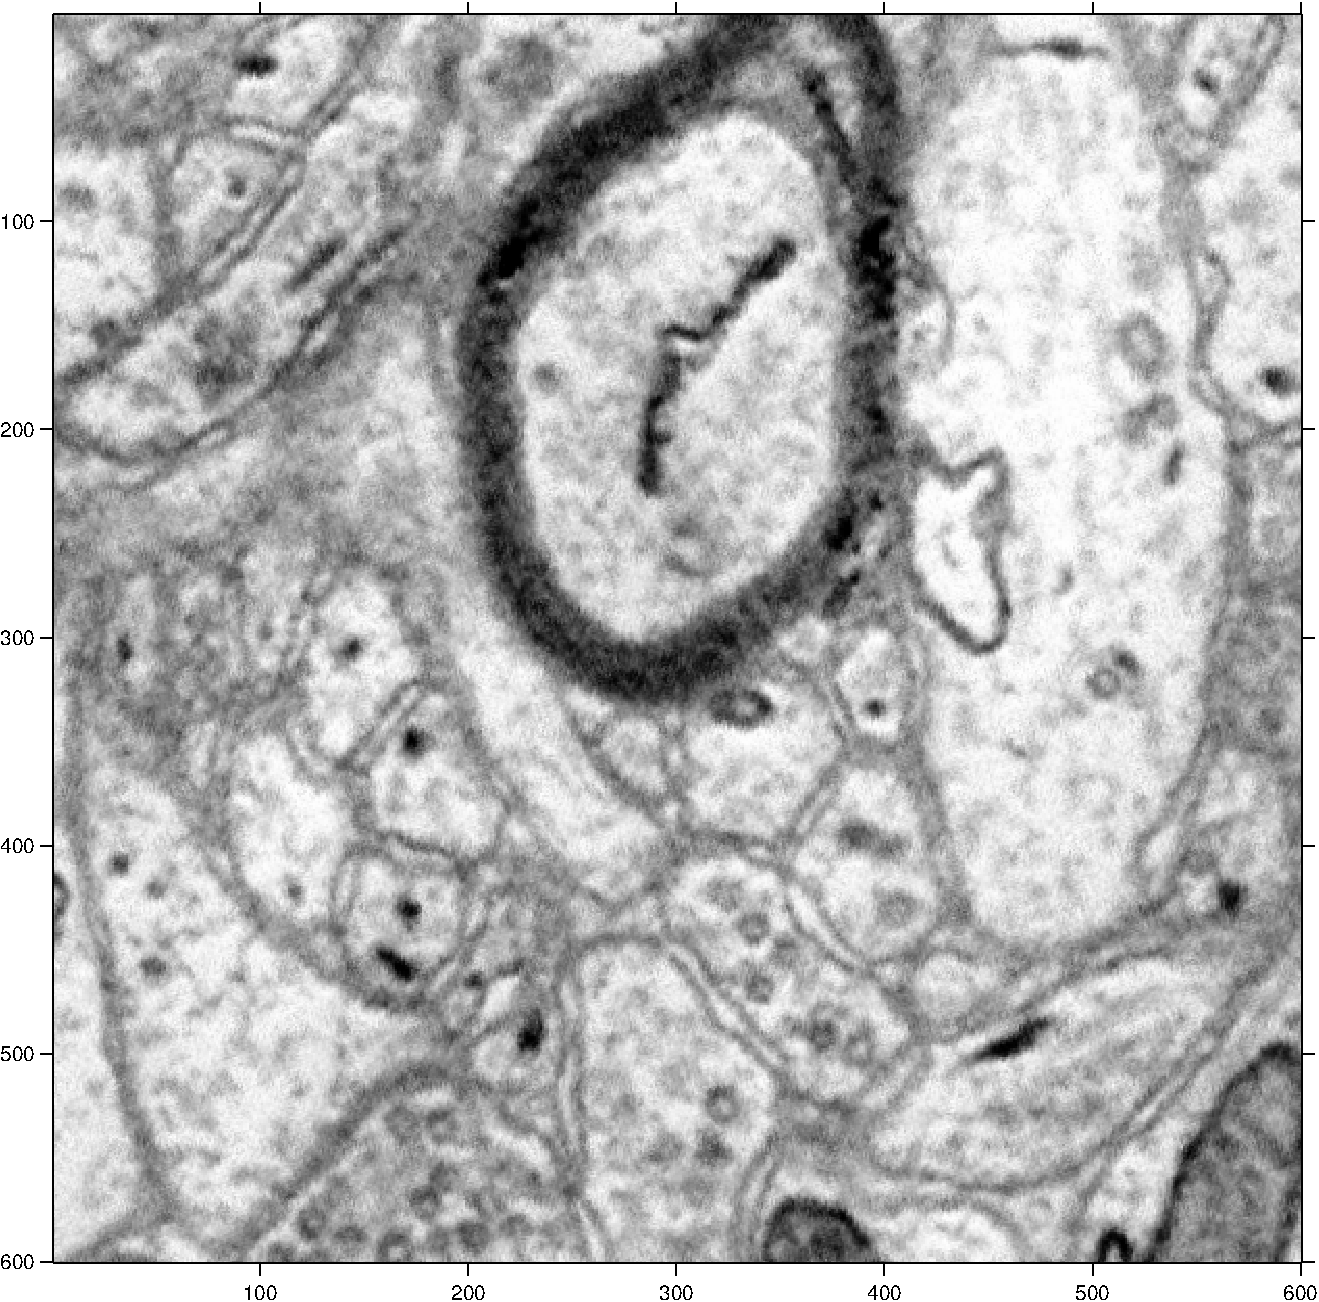
\includegraphics[width=0.32\linewidth, clip]{JAN_im}
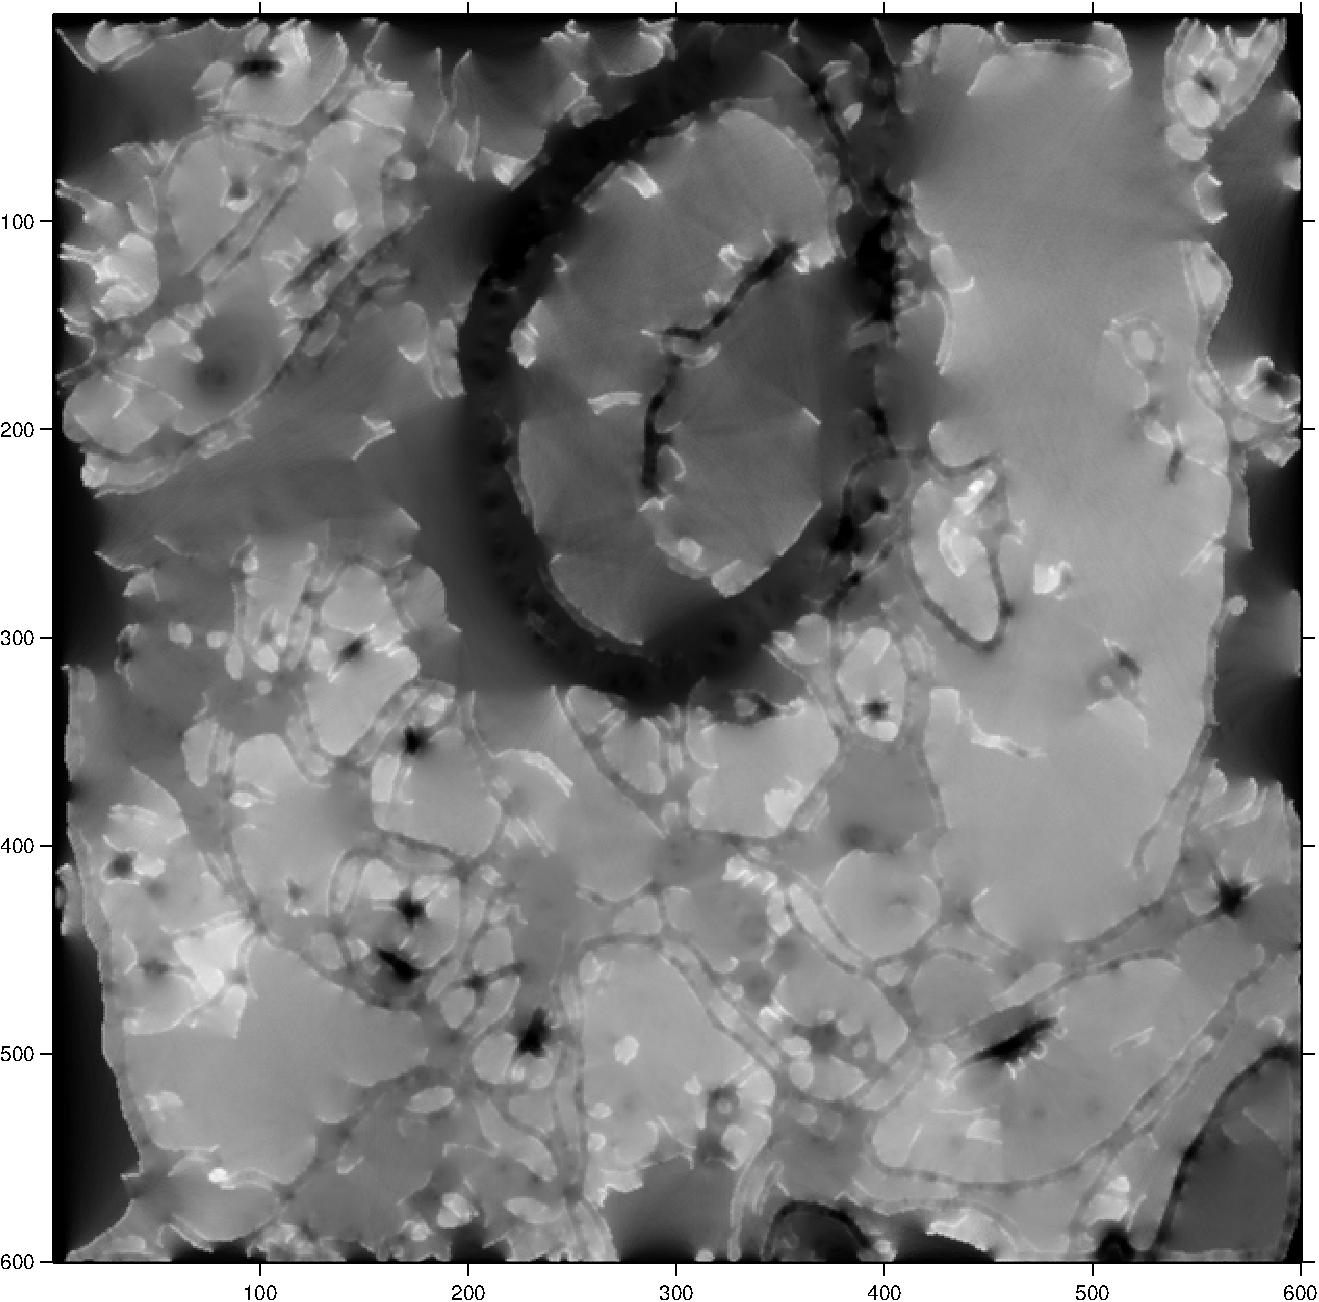
\includegraphics[width=0.32\linewidth, clip]{JAN_radon_bg}
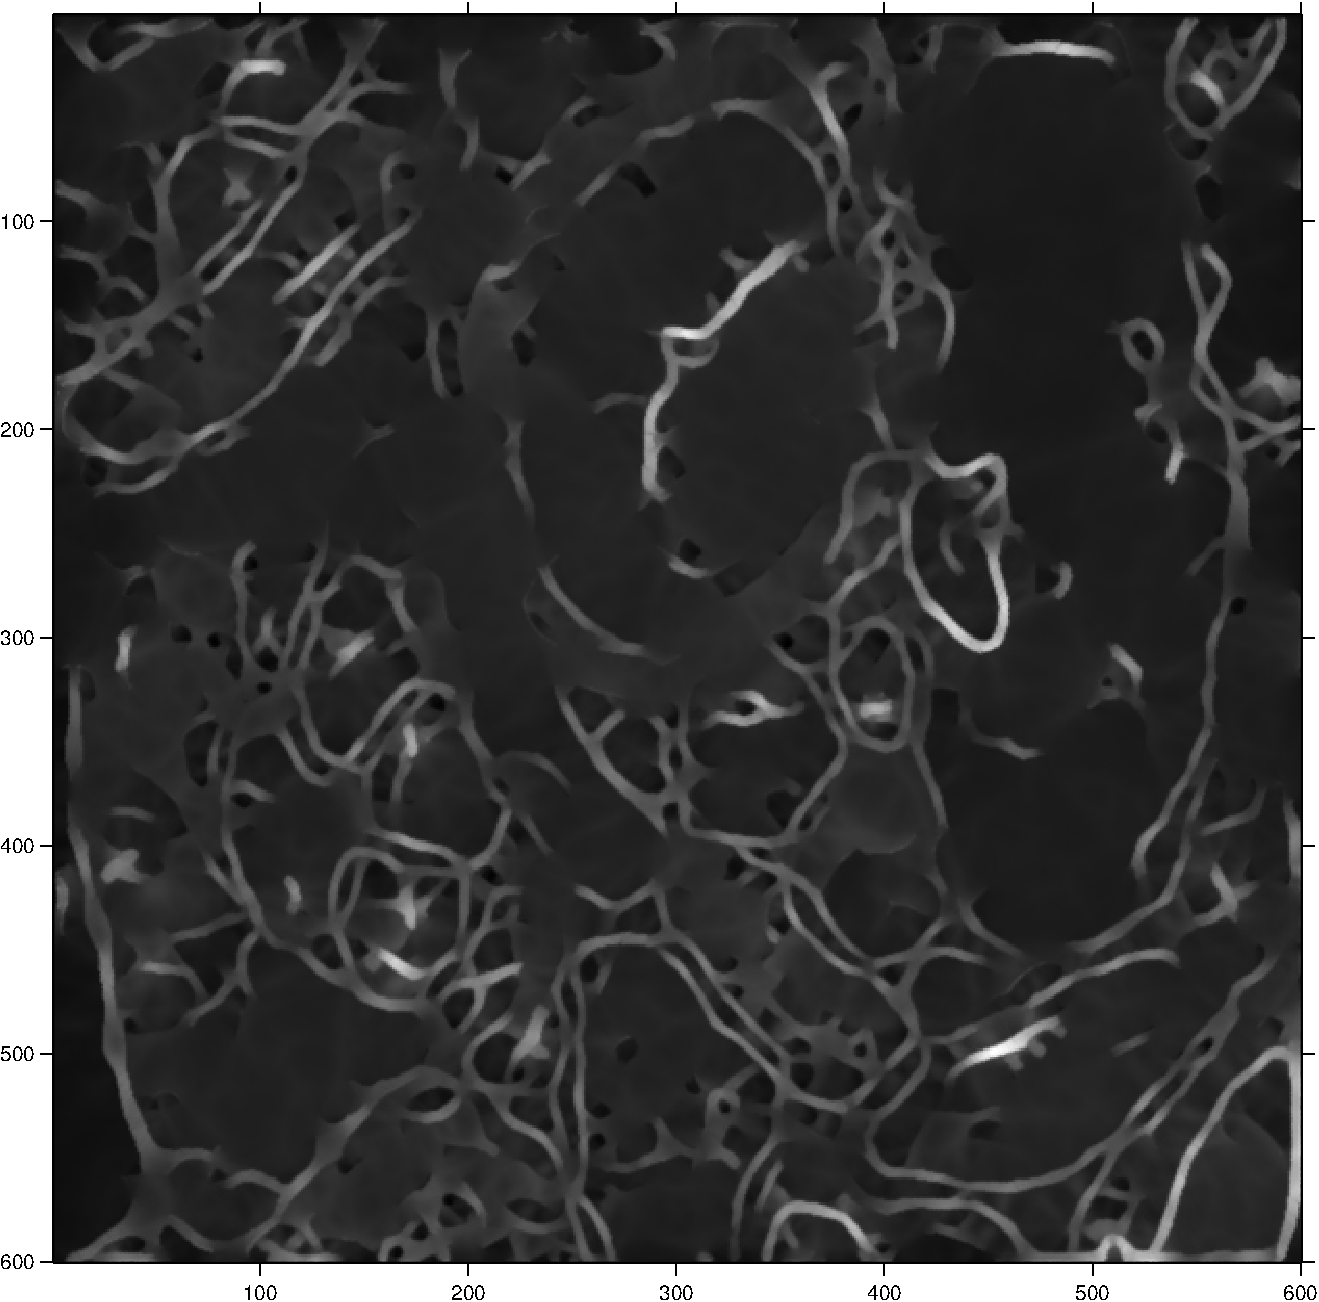
\includegraphics[width=0.32\linewidth, clip]{JAN_radon_bd}
\caption{A $600\times600$ image slice, its background average Radon response, and its boundary average Radon response. The background response homogenizes pixel intensities within a cell body, while the boundary response highlights cell boundaries.} \label{fig:radon}
\end{figure}

Ideally, for a mixture model, pixel intensities within a cell should be homogeneous. But the diversity of intracellular structures and significant imaging noise yield data far from this ideal. To correct this, we augment raw pixel intensities with $\emph{Radon-like feature}$ responses, which have proven useful for connectomics segmentation \cite{Kumar2010}. A Radon-like feature aggregates a function of image intensity over regions defined by structural constraints. Given emph{scan line} $\+{l}(t) : [0, 1] \rightarrow \+{R}^2$ denoting a direction along the image, we integrate an \emph{extraction function} piecewise, with segments defined by \emph{knots}, which are structurally salient points of the image. In particular, we determine knots as the poitns classified as edges by using a Canny edge mapper on the filter response $$R(x,y) = \max_{\sigma, \phi} \Delta G(\sigma, \phi) \ast I(x,y) $$ given in \cite{Kumar2010}, where $\Delta G(\sigma, \phi)$ is the Gaussian second derivative filter at scale $\sigma$ and orientation $\phi$. This edge response is noisy, but unlike other methods, we use it the noisy edge response only as a guide for additional feature extraction, not as a testimony for the cell segments themselves.

For a given scan line, we write its knots as parametric coordinates along the line: $K_{\+l} = \{ t_1, \ldots, t_m \}$. We follow the practice in \cite{Kumar2010} to evaluate Radon-like features along uniform angular intervals (we find 72 sufficient to avoid most discretization artifacts) and take the mean response from all directions. Of course, using the entire vector of feature responses with a multivariate likelihood is also possible. Let $T(I, x, y)$ be an extraction function which maps an image and $xy$-coordinates to a scalar. Suppose a line $\+{l}$ is given and $(x, y) = \+{l}(t)$ for some $t \in [t_i, t_{i+1}]$. Then the Radon-like response for image $I$ at $(x, y)$ in direction $\+{l}$ is given by $$\Psi \left( I,\+{l},t \right) = T \left( I, \+{l}(t) \right).$$ We will use the extraction function proposed in \cite{Kumar2010} for cell background segmentation $$T_{\text{bg}}(I, \+{l}(t)) = \min_{t \in [t_i, t_{i+1}]} \left\{ I \left( \+{l}(t) \right) \right\}$$ which simply returns the dimmest pixel between any two knots. Because knots denote edges, this feature tends to homogenize pixel intensities within a cell.

Finally, we want pixels to not cross cell boundaries. The first step in encoding this constraint is to use a boundary-enhancing extraction function \cite{Kumar2010} $$T_{\text{bd}} = \frac{\int_t^{t+1} R\left( \+{l}(\tau) \right) d\tau }{\left\Vert \+{l}(t_{i+1}) - \+{l}(t_{i}) \right\Vert_2 }.$$ This function assigns to each pixel the average value of the Gaussian second-derivative response. Recall that the GSD tends to enhance boundaries, the most salient of which are captured by the Canny detector as knots. Thus, $T_{\text{bd}}$ smoothes the spurious GSD responses, avoiding oversegmentation. Further, in connectomics data, cell membranes tend to form thick boundaries. But classic edge detectors work best at single-pixel gradients and return two edges for a thick boundary. In particular, the Canny detector produces two knots on either side of a cell boundary. In the GSD response $R$, cell boundaries are consistently bright, so the integral in $T_{\text{bd}}$ returns a distinctly brighter response on boundaries, regardless of thickness. We use this boundary enhancement information in the next section.

\subsection{Geodesic Distance}
\label{sec:geodesic}
\begin{figure}
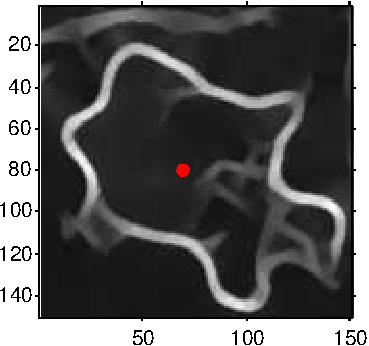
\includegraphics[width=0.24\linewidth, clip]{JAN_bd_small}
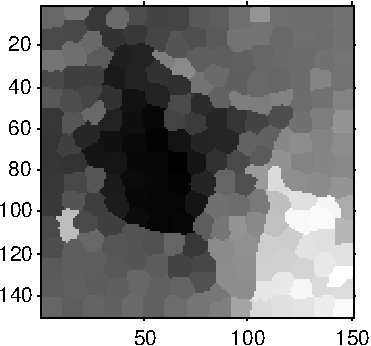
\includegraphics[width=0.24\linewidth, clip]{JAN_bd_dist}
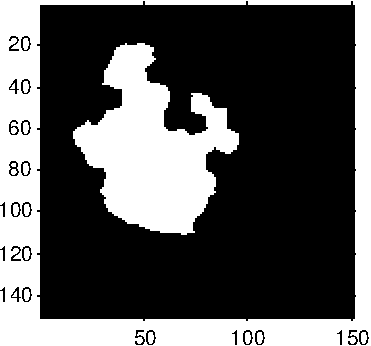
\includegraphics[width=0.24\linewidth, clip]{JAN_bd_thresh}
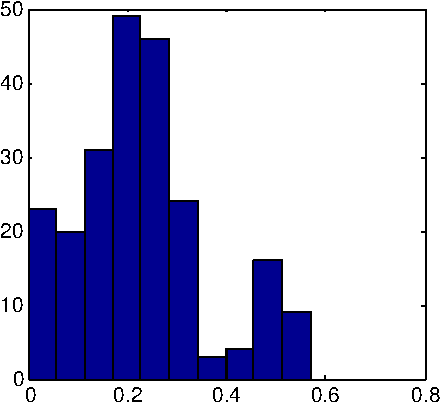
\includegraphics[width=0.24\linewidth, clip]{JAN_bd_hist}
\caption{(1) Boundary Radon-like feature response; red marks the center from which the remaining pictures are measured. (2) Grayscale map of geodesic distance (of superpixels). (3) Threshold of geodesic distance $< 0.1$. Distribution of geodesic distances about the red center.\label{fig:geodesic}}
\end{figure}
Figures~\ref{fig:radon} and~\ref{fig:geodesic} illustrate that cells need not be elliptical, or even convex. All that can be said is that they are contained in a closed loop that is generally gives a distinct Radon-like boundary response. Therefore, shape constraints based on Euclidean distances are not justified. Instead, we want to encode the a priori belief that ``the cell body should not spill outside its membrane.'' Let us quantify this statement. Construct an undirected graph with pixels as vertices and pairs of adjacent pixels as edges ($(x,y)$ is an edge if $y$ is in the 1-pixel neighborhood of $x$). Each edge has a weight $w(i,j) = \left| b_i - b_j \right|$ where $b_k$ is the boundary Radon-like response at pixel $k$. We define the \emph{geodesic distance} $d(\+{x}_i, \+{x}_j)$ to be the total weight of the shortest path between pixels $i$ and $j$, which is computed with Johnson's algorithm. In practice, the $O(N^2)$ storage is prohibitive, so we instead we downsample the image into SLIC superpixels \cite{Achanta2012} and compute superpixel-based distances. Further, because individual cells are tiny relative to an entire slice, only local distances are needed, because far points must be outside the current cell. All paths crossing a cell boundary must traverse pixels with low, high, and again low boundary feature responses. Thus, the shortest path will also be one with a high weight. So if pixels $i$ and $j$ do not belong to the same cell, defined by the region enclosed by a loop of pixels with high boundary feature response, then $d(\+{x}_i, \+{x}_j)$ is high.

Recall that the cluster mean contains entries for the $xy$-coordinates $\+{\mu}_{k,1:2} = (\mu_{k,x}, \mu_{k,y})$. Fix a point $n$ and a cluster $k$. Then $d(\+{x}_n, \+{\mu}_{k,1:2})$ is exponentially distributed, favoring distances close to zero. Any point one the opposite side of a boundary from the cluster's center will be far away from zero, and hence have low probability. Geodesic distances to other points are ignored.

\section{Inference}
Inference is performed by Gibbs sampling, using Radford Neal's Algorithm 8 for non-conjugate priors \cite{Neal2000}. This is because the likelihood of $\+x$, which depends on the function $d$, is not a known conjugate-parametric form.\fxwarning{I'm not sure this is the right explanation.} We collapse $\+\pi$, but we do not collapse the other latent variables. Denote by $X_{-n}$ the set of all $\+x_n$ with point $n$ removed, by $X_k = \left\{ \+x_n \in X : z_n = k \right\}$ and $N_k = | X_k |$. Then we derive the conditionals by finding the Markov blankets of each node and using Bayes' rule. But because the likelihood of $\+x_n$ is not a standard parametric form, conditionals involving $X_k$ and $\+\mu_k$ cannot be sampled explicitly; we can only compute their likelihoods up to proportionality and resort to Metropolis-Hastings sampling.
\begin{align}\label{eq:conds}
p(z_n = k | \+\pi, \+x_n, \+\mu_k, \Lambda_k) &\propto p(z_n = k | \+\pi) \mathcal{N}(\+x_n | \+\mu_k, \Lambda_k) \label{eq:z}\\
p(\gamma_k | X_k, \+\mu_k, \beta_0, \gamma_0) &= \text{Gamma}\left( \gamma_k | \beta_0 + N_k, \gamma_0 + \sum_{\+x \in X_k} d(\+x, \+\mu_k) \right) \label{eq:gamma}\\
p(\Lambda_k | X_k, \+\mu_k, \gamma_k, \Lambda_0, \nu) &\propto  p(X_k | \+\mu_k, \Lambda_k, \gamma_k) \text{Wishart}(\Lambda_k | \Lambda_0, \nu) \label{eq:lambda}\\
p(\+\mu_k | X_k, \Lambda_k, \gamma_k, \+\mu_0, \kappa) &\propto p(X_k | \+\mu_k, \Lambda_k, \gamma_k) \mathcal{N}(\+\mu_k | \+\mu_0, (\kappa\Lambda)^{-1}) \label{eq:mu}
\end{align}
Note that $\+\pi$ remains collapsed; to evaluate \eqref{eq:z}, see \eqref{eq:mdp}.

\begin{algorithm}
\caption{Gibbs sample sweep}\label{alg:gibbs}
\begin{algorithmic}
\Require The current state of the Markov chain, $\Theta = \left\{ N, K, Z, \left\{ N_k, \+\mu_k, \Lambda_k, \gamma_k \right\}_{k=1}^K  \right\}$
\Statex

\For{$n := 1:N$}
  \If{$N_{z_n} = 1$}
    \State $\left( \+\mu_{K+1}, \Lambda_{K+1}, \gamma_{K+1} \right) := \left( \+\mu_{K+1}, \Lambda_{K+1}, \gamma_{K+1} \right)$ 
    \State Draw $\+\mu_j, \Lambda_j, \gamma_j$ from their priors (see section~\ref{sec:model}), for $j \in \{K+2, \ldots, K+m\}$
  \Else
    \State Draw $\+\mu_j, \Lambda_j, \gamma_j$ from their priors (see section~\ref{sec:model}), for $j \in \{K+1, \ldots, K+m\}$
  \EndIf
  \State Draw $z_n$ from 
  \[
  p(z_{n}=k|\+{z}_{-n},X_{-n},\alpha,\left\{ \+\mu_k,\Lambda_k,\gamma_k\ \right\}_{k=1}^{\infty}) \propto \begin{cases}
  \frac{N_{k,-n}}{N-1+\alpha} p(\+x_n | \+\mu_k, \Lambda_k, \gamma_k) & k < K\\
  \frac{\alpha / m}{N-1+\alpha} p(\+x_n | \+\mu_k, \Lambda_k, \gamma_k) & \text{otherwise}
  \end{cases} \label{eq:nealalg8}
  \]
  \State Delete parameters for classes $k$ with $N_k = 0$ and relabel the $z_n$ to remove gaps.
\EndFor

\For{$k := 1:K$}
  \State Draw $\gamma_k$ using \eqref{eq:gamma}
  \State Metropolis-Hastings sample $\Lambda_k$ using likelihood \eqref{eq:lambda} and proposal $\text{Wishart}(\Lambda^{*} | b \Lambda, \nu)$ for some $b > 1$.
  \State Metropolis-Hastings sample $\+\mu_k$ using likelihood \eqref{eq:mu} and proposal $\mathcal{N}( \+\mu^{*} | C )$.
\EndFor

\end{algorithmic}
\end{algorithm}

\subsection{Proposal Distributions}
Care is required to select proposal distributions for \eqref{eq:mu}, because the likelihood for $\+x_n$ is discontinuous in $\+\mu_k$, since it relies on the discrete function $d$ which arises from graph distances. The lack of reliable gradient information frustrates the smooth exploration of low-probability areas. However, discontinuities only occur at superpixel boundaries, and sharp discontinuities only at the transition between cell boundary and interior. Therefore, we use a diagonal-covariance Gaussian proposal whose $xy$ coordinate marginal forms a 95\% confidence ellipse that covers the neighboring superpixels. SLIC superpixels have roughly uniform size, even if shapes differ. Thus, a circle can be guaranteed to cover some neighbors of a superpixel. Thus, we propose with the following covariance
\[
C = \left(\begin{array}{cccc}
    \sigma^{2} & & & \text{\huge 0}\\
     & \sigma^{2} & & \\
      &  & \tau^{2} &\\
    \text{\huge 0} &  &  & \tau^{2}
     \end{array}\right)
\]
where $\sigma$ is the diameter of a SLIC superpixel and $\tau = 1/2$, because the third and fourth features are constrained to lie in $[0, 1]$.

To sample $\Lambda_k$, since $\+\mu_k$ is constant, equation \eqref{eq:lambda} is continuous in $\Lambda_k$, so a Wishart proposal suffices. However, to ensure exploration of the state space, we adjust the variance of the Wishart proposal to be higher than in the prior in \ref{sec:model}.

\section{Results}
Forthcoming.

\section{Discussion}
Forthcoming.

\appendix
\section{Dirichlet Process Mixtures}
\label{sec:mdp}
We begin with a finite Gaussian mixture model and derive the Dirichlet process mixture as a limiting case. This follows the derivation first given by \cite{Rasmussen2000}.

The $N$ observations are divided among $K$ classes. We record the class membership of $\+{x}_n$ with a latent indicator $z_n \in \{1, \ldots, K \}$. Given a class assignment $z_n = k$, we assume $x_n$ is drawn from a distribution $F(\+{x}|\Theta_k)$ where $\Theta_k$ is a vector of parameters. Therefore, a mixture model gives each class its own parameter vector, but assumes that observations are conditionally independent given a class.

The indicators $z_n$ are drawn from the discrete distribution $\+\pi$, a $K$-dimensional vector which is in turn is drawn from a symmetric Dirichlet distribution parameterized by $\alpha$: $$p \left( \+\pi | \alpha, K \right) = \frac{ \Gamma ( \alpha ) }{ \Gamma ( \alpha/K ) ^K} \prod_{k=1}^K \+\pi_k^{\alpha/K - 1}.$$ Because the Dirichlet and discrete distributions are conjugate, we can marginalize $\+\pi$. Let $\+{z}_{-n}$ denote the vector of all indicators excluding element $n$ and $N_{k,-n}$ denote the number of points assigned to class $k$ excluding point $n$. A standard result \cite{Rasmussen2000} yields the posterior $$p(z_n = k | \+{z}_{-n})  = \frac{ N_{k,-n} + \alpha/K }{ N - 1 + \alpha }.$$

Now consider $K \rightarrow \infty$. First, the term $\alpha / K \rightarrow 0$. Given finitely many observations, we have only finitely many components $k$ with $N_{k,-n} > 0$. Therefore, the density 
\[
p(z_{n}=k|\+{z}_{-n},\alpha)=\begin{cases}
\frac{N_{k,-n}}{N-1+\alpha} & N_{k,-n}>0\\
\frac{\alpha}{N-1+\alpha} & \text{otherwise}
\end{cases} \label{eq:mdp}
\]
satisfies the limiting conditions and correctly normalizes to 1 when summed over $k = 1, \ldots, \infty$. The mixing distribution $\+\pi$, which is now infinite-dimensional, can also be said to be drawn from a \emph{Dirichlet process}. It is known that even the infinite-dimensional case conjugacy allows us to eliminate $\+\pi$ from computations, making Gibbs sampling from an infinite mixture is just as efficient as for a finite mixture case.

\bibliographystyle{plain}
\bibliography{refs.bib}
\end{document}
